\chapter{Конструкторский раздел}

В данном разделе представлены схемы алгоритма поиска минимального элемента в матрице последовательным способом и с помощью параллельной реализации. Было выполнено описание способов тестирование и выделенных классов эквивалентностей. Также представлены выбранные типы и структуры данных.

\section{Выбранные типы и структуры данных}
В данной работе используются следующие типы и структуры данных:
\begin{itemize}
	\item matrix\_args\_t - структура, содержащая матрицу, количество строк и столбцов в ней;
	\item pthread\_args\_t - структура, содержащая информацию о номере потока, количестве потоков, количестве строк матрицы, локальный минимум и структуру matrix\_args\_t.
\end{itemize}

\section{Схемы алгоритмов}
Ниже представлены следующие схемы алгоритмов:
\begin{itemize}
	\item рисунок \ref{png:1} - схема алгоритма поиска минимума в матрице (последовательная реализация);
	\begin{figure}[H]
		\centering{
			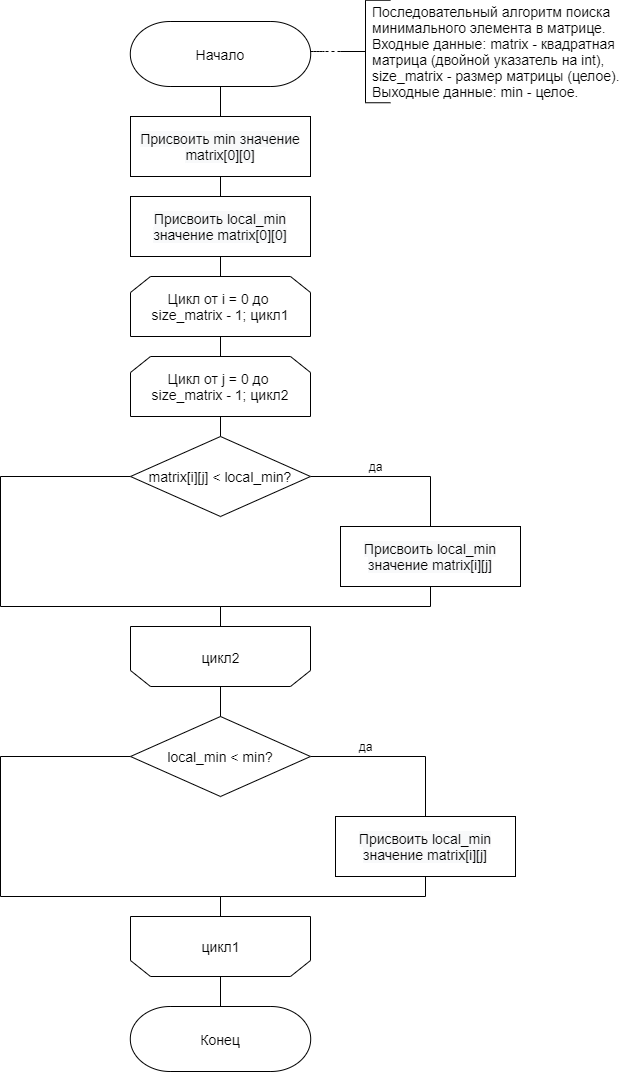
\includegraphics[scale=0.6]{../../../../../../../msys64/home/Лев/bmstu_sem_5_aa/lab_04/report/diagrams/sequential}
			\caption{Схема алгоритма поиска минимума в матрице (последовательная реализация).}
			\label{png:1}}
	\end{figure}

	\newpage
	\item рисунок \ref{png:2} - схема алгоритма поиска минимума в матрице (параллельная реализация);
	\begin{figure}[H]
		\centering{
			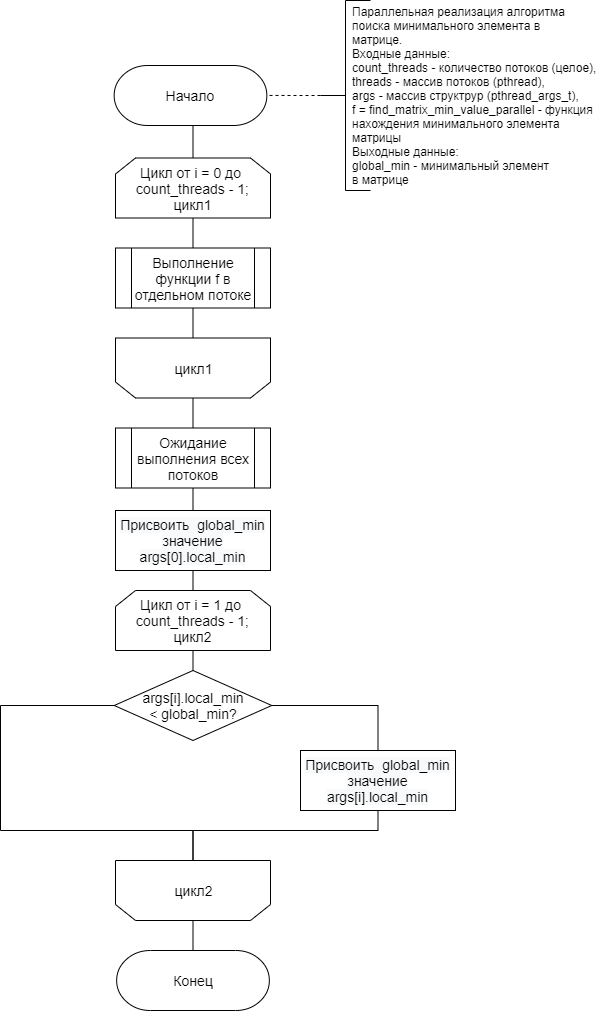
\includegraphics[scale=0.6]{../../../../../../../msys64/home/Лев/bmstu_sem_5_aa/lab_04/report/diagrams/parallel_1}
			\caption{Схема алгоритма поиска минимума в матрице (параллельная реализация).}
			\label{png:2}}
	\end{figure}

	\item рисунок \ref{png:3} - распределение задач поиска минимума в матрице (параллельная реализация);
	\begin{figure}[H]
		\centering{
			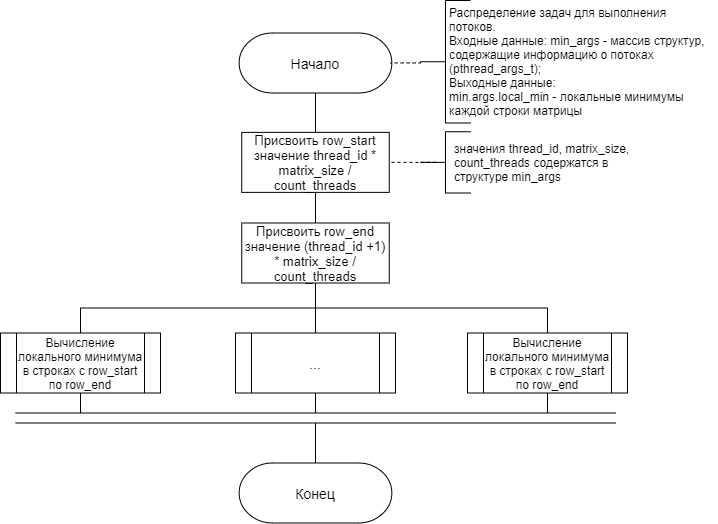
\includegraphics[scale=0.6]{../../../../../../../msys64/home/Лев/bmstu_sem_5_aa/lab_04/report/diagrams/parallel_2}
			\caption{Распределение задач поиска минимума в матрице (параллельная реализация).}
			\label{png:3}}
	\end{figure}
\end{itemize}

\section{Вывод}
На основе теоретических данных, полученных в аналитическом разделе, были построены схемы необходимых реализаций алгоритма, представлены необходимые типы и структуры данных.